% Created 2026-10-14 Wed 09:09
% Intended LaTeX compiler: pdflatex
\documentclass[preprint,12pt]{elsarticle}
\usepackage{graphicx}
\usepackage{rotating}
\journal{Computer Physics Communications}
\usepackage{iftex}
\ifPDFTeX\usepackage[utf8]{inputenc}\usepackage[T1]{fontenc}\usepackage{lmodern}\else\usepackage{fontspec}\fi
\usepackage{microtype}
\makeatletter
% The class footer box is followed by a space token.
% The output routine then packs that box to \textwidth, and the space makes the line 2.6pt overfull.
\def\ps@pprintTitle{%
\let\@oddhead\@empty
\let\@evenhead\@empty
\def\@oddfoot{%
\hbox to \textwidth{%
\ifnopreprintline\relax\else
\@myfooterfont
\ifx\@elsarticlemyfooteralign\@elsarticlemyfooteraligncenter
\hfil\@elsarticlemyfooter\hfil
\else
\ifx\@elsarticlemyfooteralign\@elsarticlemyfooteralignleft
\@elsarticlemyfooter\hfill{}%
\else
\ifx\@elsarticlemyfooteralign\@elsarticlemyfooteralignright
{}\hfill\@elsarticlemyfooter
\else
Preprint submitted to \ifx\@journal\@empty
Elsevier%
\else\@journal\fi\hfill\@date\fi
\fi
\fi
\fi
}%
}%
\let\@evenfoot\@oddfoot}
\makeatother
\usepackage{amssymb,amsmath}
\setlength{\emergencystretch}{2em}
\usepackage{booktabs}
\usepackage{listings}
\usepackage{xurl}
\usepackage{xcolor}
\usepackage{hyperref}
\usepackage{xr-hyper}
\makeatletter
\let\readcon@bibcite\bibcite
\def\bibcite#1#2{}%
\externaldocument{rg_main}
\let\bibcite\readcon@bibcite
\makeatother
\input{affilfix}
\lstset{
basicstyle=\ttfamily\footnotesize,
breaklines=true,
breakatwhitespace=false,
columns=fullflexible,
keepspaces=true,
showstringspaces=false,
frame=none,
aboveskip=0.6em,
belowskip=0.4em
}
\renewcommand{\thesection}{S\arabic{section}}
\renewcommand{\thetable}{S\arabic{table}}
\renewcommand{\thefigure}{S\arabic{figure}}
\AtBeginDocument{\renewcommand{\thelstlisting}{S\arabic{lstlisting}}}
\hypersetup{colorlinks=true,linkcolor=black,citecolor=black,urlcolor=blue!50!black}
\date{\today}
\title{Supplementary material: CON 3.1}
\hypersetup{
 pdfauthor={Rohit Goswami},
 pdftitle={Supplementary material: CON 3.1},
 pdfkeywords={restart, specification, saddle search, conformance},
 pdfsubject={},
 pdflang={English}}
\begin{document}

\label{sec:org49296de}
\begin{frontmatter}
\input{authors.tex}
\begin{abstract}
These notes record the measurements behind the CON 3.1 paper.
The restart displacements, the format matrix, the frame bytes, the velocity step and the illegal-file classes are the campaign results and the conformance corpus.
The language-pair table and the MPI rank tables are the distributed campaign.
The ingest tables are the readcon-db 0.1.8 evaluation.
The archived store release is 0.2.0.
\end{abstract}
\end{frontmatter}
\section{Restart difference}
\label{sec:supp-restart}
The interrupted band in Section \ref{sec:cases} writes a checkpoint and then continues.
Figure \ref{fig:supp-restart} compares each resumed movie with the uninterrupted movie at the same index.
Column 3 is that checkpoint.
The final column is the band after the five steepest-descent steps.

\begin{figure}[ht]
\centering
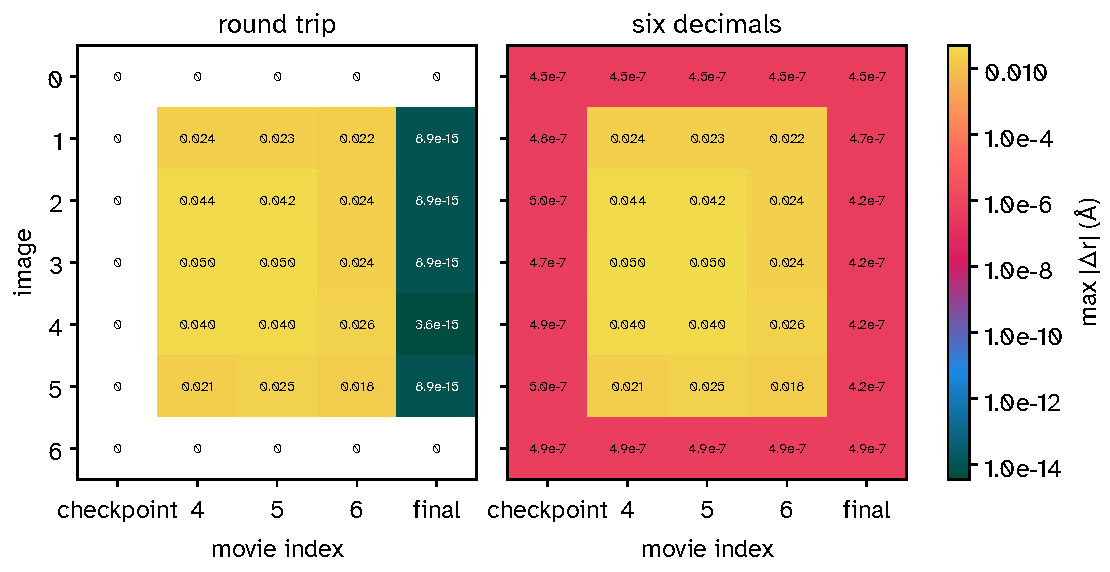
\includegraphics[width=\textwidth]{figures/generated/restart_diff.pdf}
\caption{Minimum-image maximum component of the displacement, in \AA, between the uninterrupted Morse band and each resume.
The checkpoint column is bitwise exact for the round-trip printer and \(4.90\times10^{-7}\,\text{\AA}\) for six decimals.
The final column is at most \(8.9\times10^{-15}\,\text{\AA}\) for the round trip and \(4.9\times10^{-7}\,\text{\AA}\) for six decimals.
Intermediate columns differ by up to \(0.050\,\text{\AA}\) because the search has taken further steps after the load.}
\label{fig:supp-restart}
\end{figure}
\section{Round-trip fidelity}
\label{sec:supp-fidelity}
Figure \ref{fig:supp-fidelity} uses two unmodified files.
The matrix rows other than the velocity-file row are the first frame of the height-held EMT band.
That frame already carries mask 4, a \(z\)-only hold, on the adatom, together with ids, forces and an energy.
It carries no velocities and no time unit, so the time-unit cell on those rows is absent.
The velocity-file row is a separate round trip of the unmodified 28-atom velocity fixture, whose time unit is the natural unit.
Neither file was edited.
The grades are the fields that come back from a write and a read.

\begin{figure}[ht]
\centering
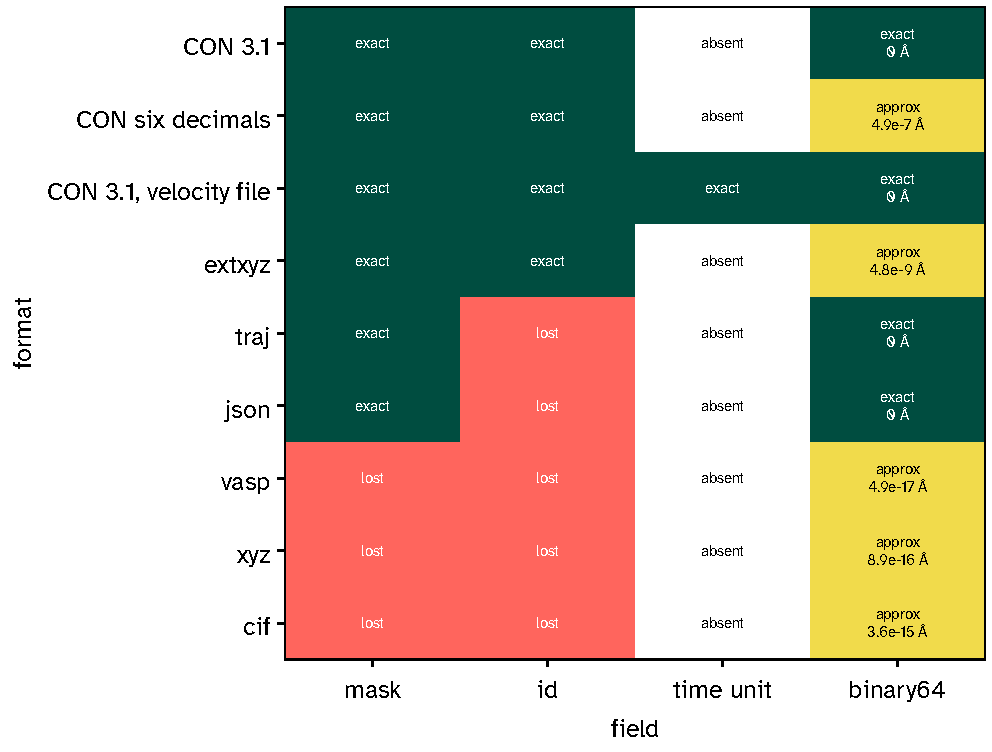
\includegraphics[width=0.92\textwidth]{figures/generated/roundtrip_fidelity.pdf}
\caption{Fields kept by a write and a read.
The held-frame rows have no time unit in the source file.
The velocity-file row keeps the natural unit.
CON 3.1 keeps the mask, the id and binary64 on both files.
Six decimals keep the mask and the id and move a held-frame coordinate by \(4.9\times10^{-7}\,\text{\AA}\).
Extended XYZ keeps the mask and the id and moves a coordinate by \(4.8\times10^{-9}\,\text{\AA}\).
The trajectory and JSON writers keep the mask and the coordinates and drop the id.
POSCAR, XYZ and CIF drop the mask and the id.
The number in the binary64 cell is the maximum absolute coordinate change.
A grey cell is a time unit the source frame did not carry.}
\label{fig:supp-fidelity}
\end{figure}
\section{Frame bytes and parse time}
\label{sec:supp-anatomy}
The frame is the 28-atom velocity file, 3,826 bytes.
The timed files are 400 copies of that frame and 400 copies with the velocity section removed.
The reported times are medians of 31 paired reads.
Figure \ref{fig:supp-anatomy} is the byte width of each span and the parse time of those files.

\begin{figure}[ht]
\centering
\includegraphics[width=\textwidth]{figures/generated/frame_anatomy.pdf}
\caption{Byte widths of one CON 3.1 frame, and the parse time of the same spans.
Masks, ids and the time unit are 227 bytes, against 1{,}429 coordinate bytes and 1{,}860 velocity-number bytes.
The velocity section adds \(2.90\,\mu\mathrm{s}\) to a \(13.2\,\mu\mathrm{s}\) read of the rest of the frame.
Masks and ids share the coordinate line, so their parse time is inside that \(13.2\,\mu\mathrm{s}\).}
\label{fig:supp-anatomy}
\end{figure}
\section{Velocity mislabel}
\label{sec:supp-velocity}
The kinetic energies and the Verlet step are the illustration in Section \ref{sec:cases}.
The conversion from the natural unit to femtoseconds is \(10.180505710759414\,\mathrm{fs}\), and the kinetic factor is its square.
The cell is the slab cell of the file.
Figure \ref{fig:supp-velocity} is the displacement after that step.

\begin{figure}[ht]
\centering
\includegraphics[width=\textwidth]{figures/generated/velocity_mislabel.pdf}
\caption{Displacement after one velocity Verlet step of \(1\,\mathrm{fs}\) on the 28-atom slab when the natural velocity is misread as \(\text{\AA}/\mathrm{fs}\).
The kinetic energy goes from \(0.888\,\mathrm{eV}\) to \(92.02\,\mathrm{eV}\), a factor of 103.64.
The RMSD is \(0.096\,\text{\AA}\) and the maximum component is \(0.315\,\text{\AA}\).
The arrows are drawn at 10 times that displacement.}
\label{fig:supp-velocity}
\end{figure}
\section{Illegal-file classes}
\label{sec:supp-errors}
These are the eight illegal files from the corpus in Section \ref{sec:conformance}.
The corpus also holds 10 legal files.
readcon raises a message that names the class.
ASE 3.29.0 reads the same files with its eon reader.
Figure \ref{fig:supp-errors} is the class of each file.

\begin{figure}[ht]
\centering
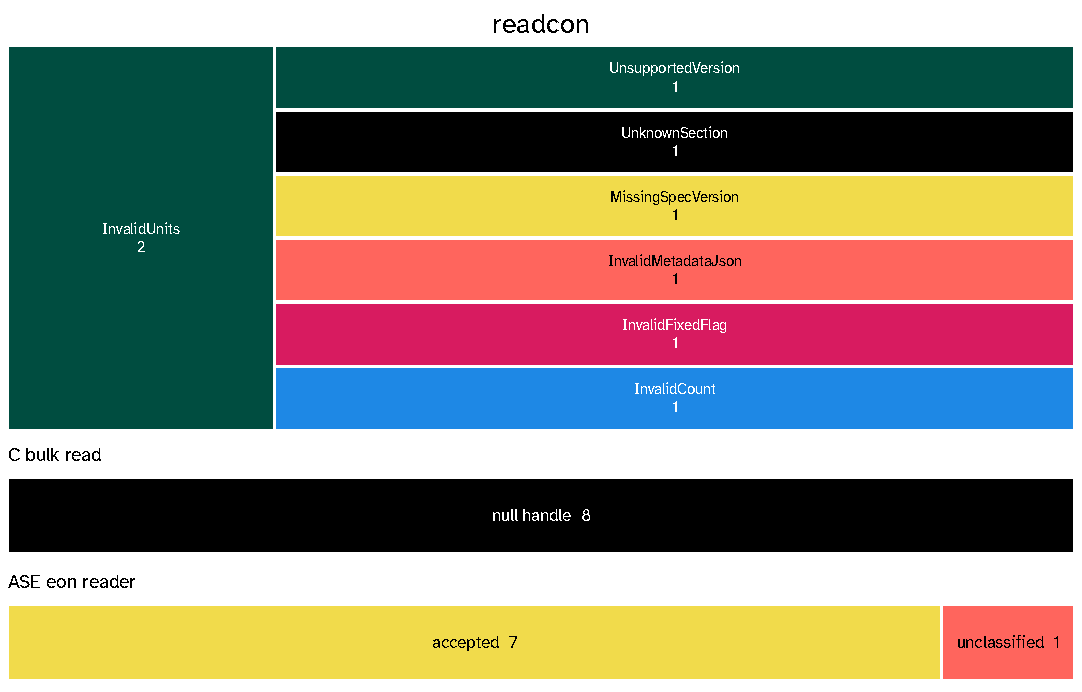
\includegraphics[width=\textwidth]{figures/generated/error_classes.pdf}
\caption{Classes on the eight illegal files.
readcon names a class for each file.
The ASE eon reader accepts seven of the files and stops without a class on the per-type count of zero.}
\label{fig:supp-errors}
\end{figure}
\section{Database hashes of the campaign bands}
\label{sec:supp-dedup}
The hashes are a query against readcon-db 0.1.8.
The five bands were appended as stored trajectories, and each frame hash was read back by the same query.
The bands are the uninterrupted Morse restart, its round-trip resume, its six-decimal resume, and the two EMT mask bands of Section \ref{sec:cases}.
The query returns 35 images and 35 hashes.
Every returned hash locates the frame that was stored.
Endpoint coordinates of the uninterrupted band and the round-trip resume agree: the maximum absolute component is 0 at both endpoints and \(8.9\times10^{-15}\,\text{\AA}\) over the seven images.
The stored texts still differ, so the hash keeps every frame apart.
On the reactant the only differing line is the metadata line.
The printed curvature products differ by one byte, 2,507 bytes against 2,506, and the coordinate rows match.
The product frame differs only in that same metadata line.
The five intermediate images differ in the metadata line and in coordinate rows at the last printed digits, which is the \(8.9\times10^{-15}\,\text{\AA}\) displacement.
Figure \ref{fig:supp-dedup} is the query: 35 images and 35 hashes, with no hash shared.
Figure \ref{fig:supp-neb} is the same five bands on the \((s, d)\) plane \cite{goswamiTwodimensionalRmsdProjections2026}.

\begin{figure}[ht]
\centering
\includegraphics[width=0.86\textwidth]{figures/generated/dedup_graph.pdf}
\caption{Campaign bands on the left and the database hash of each stored frame on the right.
The query returns 35 images and 35 hashes.
No hash is shared.
The endpoints match in coordinates.
Their hashes differ because the metadata line does.}
\label{fig:supp-dedup}
\end{figure}

\begin{figure}[ht]
\centering
\includegraphics[width=\textwidth]{figures/generated/neb_multiples.pdf}
\caption{The same five bands on the \((s, d)\) plane \cite{goswamiTwodimensionalRmsdProjections2026}.
The Morse maps share one colour scale and the EMT maps share another.
Black dots are the images.
The round-trip and six-decimal maps sit on the uninterrupted Morse band at this scale.}
\label{fig:supp-neb}
\end{figure}
\section{Failure cases: frame, grading and drift files}
\label{sec:supp-failure}
The survey frame is a Pt(100) \(2\times2\times2\) slab with 6\hspace*{.2em}\AA{} of vacuum and one Pt adatom 1.8\hspace*{.2em}\AA{} above the hollow site.
Every coordinate carries a uniform offset of up to \(10^{-3}\,\text{\AA}\) from a fixed seed, so all seventeen significant digits are needed.
The bottom four atoms are fixed on every axis, and the adatom is fixed in \(z\).
The ids are 17, 3, 11, 5, 23, 2, 13, 7 and 41 in row order.
Velocities are normal deviates of standard deviation \(4\times10^{-3}\) in the natural unit, zero on held axes.
For ASE the masks become one FixAtoms and one FixCartesian, the ids an integer array named \texttt{id}, and the velocities ASE momenta.
For MDAnalysis the velocities are converted to \(\text{\AA}/\mathrm{ps}\), its base unit.
We count a field as kept when it reads back equal; a mask counts as a full freeze when every masked atom returns frozen on every axis.
A velocity is declared when the file names its unit and the values agree after conversion to within \(10^{-6}\) relative.
When the file names no unit, we report what a reader that takes the numbers as \(\text{\AA}/\mathrm{fs}\) would see, a kinetic energy 103.64 times too large.

Each drift file has three Pt atoms with the header
\begin{lstlisting}
Lattice="5.5437171645025325 0.0 0.0 0.0 5.5437171645025325 0.0 0.0 0.0 20.0" Properties=species:S:1:pos:R:3:move_mask:L:3:id:I:1 pbc="T T F"
\end{lstlisting}
and rows \texttt{Pt 0.0 0.0 6.0 T T T 17}, \texttt{Pt 2.7718585822512662 0.0 6.0 T T T 3} and \texttt{Pt 1.3859292911256331 1.3859292911256331 7.8 F F T 41}.
The variants drop the \texttt{pbc} key, replace the header by a plain comment and the rows by their first four fields, write the \(z\) value 6.0 as \texttt{6.0d0}, spell the booleans \texttt{True} and \texttt{False}, add \texttt{note="E=1.5 eV"}, and add \texttt{units="angstrom,eV,fs"}.
The readers are ASE 3.29.0, the libAtoms extended XYZ parser through its C path and its Python path, chemfiles 0.10.4, and MDAnalysis 2.10.0.
The correctly rounded binary64 value of 2.7718585822512662 has the bit pattern \texttt{40062cc4313f3fb9}; chemfiles returns \texttt{40062cc4313f3fb8}.

The resume study uses an EMT Pt(100) \(3\times3\times3\) slab with 6\hspace*{.2em}\AA{} of vacuum, the bottom layer held, and one adatom 1.75\hspace*{.2em}\AA{} above a hollow and held in \(z\), hopping to the neighbouring hollow.
Endpoints were relaxed with BFGS to \(0.002\,\mathrm{eV/\text{\AA}}\).
Five movable images were interpolated with the constraints applied.
The band uses the improved tangent with a climbing image, and each step adds \(0.02\,\text{\AA}^2/\mathrm{eV}\) times the projected force.
We interrupt after step 25.
Each route writes all seven images and reads them back with the reader the route names, keeping whatever constraints and periodicity that reader returns.
\section{Reader rules}
\label{sec:appendix-rules}
Table \ref{tab:rules} collects the edge cases a reader applies.
They are the classes of Section \ref{sec:format}, stated as input and outcome.

\begin{table}[ht]
\centering
\small
\caption{Reader rules for flags, versions, identity and incomplete input.}
\label{tab:rules}
\begin{tabular}{@{}p{0.46\linewidth}p{0.46\linewidth}@{}}
\toprule
Input & Rule \\
\midrule
Column 4 outside the legal set & Illegal flag. \\
Version 1 column 4 equal to 1 & Fixed on \(x\), \(y\) and \(z\). \\
Version 1 column 4 other than 0 or 1 & Illegal flag. \\
Missing id column & Id is the zero-based row index. \\
Repeated id & File order is kept. \\
Unique ids & Ascending id is the pre-grouping order. \\
Unknown major & Rejected. \\
Unknown minor of a known major & Accepted. \\
Unknown metadata key & Kept on rewrite. \\
Unknown section at this minor & Rejected. \\
Unknown section at a newer minor, width declared & May be skipped. \\
Non-finite number & Rejected. \\
Type count of zero & Legal empty frame. \\
Short header or short section & No partial frame is returned. \\
Empty first header line & User line, kept. \\
Empty second header line & Implicit version 1. \\
Blank line after a frame, no velocity block & Line 1 of the next frame. \\
Several gzip members & Read in order. \\
\bottomrule
\end{tabular}
\end{table}
\section{Paired peer timings on every payload}
\label{sec:appendix-peers}
Table \ref{tab:ratios} extends the peer table of the main text to the 1-frame and 100-frame files.
The comparison calls the Python binding with one worker, and ASE, chemfiles, MDAnalysis and h5py run in the same process with OpenMP and BLAS limited to one thread.
XYZ and H5MD peers receive the coordinates of the same frames, written before the timed loop starts.
Each cell is one-worker readcon-core, then the peer, thirty times, after one untimed call of each side.
A repeat over 240\hspace*{.2em}s would be recorded as a timeout and a peer that raises as a failure; neither occurred.
The interval is a bias-corrected and accelerated bootstrap of the median with 9999 draws \cite{efronBetterBootstrapConfidence1987}.
On one frame the fixed cost of opening the file dominates, which is why h5py and chemfiles lose their lead there.

% Written by paper/cpc/scripts/gen_tables.py.
\begin{table}[ht]
\centering
\small
\caption{Paired time ratios. The ratio is the readcon-core time divided by the peer time, so a value below 1 means readcon-core finished sooner. The interval is a bias-corrected and accelerated 95 percent interval of the median. Failures stay in the table and are not converted into times.}
\label{tab:ratios}
\footnotesize
\setlength{\tabcolsep}{4pt}
\begin{tabular}{llrrrr}
\toprule
Payload & Peer & OK & Fail & Ratio & Interval \\
\midrule
1 frame & ASE eon & 30 & 0 & 0.135 & [0.132, 0.137] \\
1 frame & chemfiles XYZ & 30 & 0 & 0.73 & [0.726, 0.733] \\
1 frame & h5py & 30 & 0 & 0.319 & [0.316, 0.321] \\
1 frame & MDAnalysis H5MD & 30 & 0 & 0.02 & [0.0197, 0.021] \\
100 frames & ASE eon & 30 & 0 & 0.178 & [0.178, 0.179] \\
100 frames & chemfiles XYZ & 30 & 0 & 1.11 & [1.11, 1.12] \\
100 frames & h5py & 30 & 0 & 11 & [11, 11] \\
100 frames & MDAnalysis H5MD & 30 & 0 & 0.0909 & [0.0897, 0.093] \\
10000 frames & ASE eon & 30 & 0 & 0.253 & [0.251, 0.256] \\
10000 frames & chemfiles XYZ & 30 & 0 & 1.58 & [1.57, 1.6] \\
10000 frames & h5py & 30 & 0 & 47.6 & [46.7, 48.5] \\
10000 frames & MDAnalysis H5MD & 30 & 0 & 0.16 & [0.157, 0.162] \\
Pt slab & ASE eon & 30 & 0 & 0.215 & [0.211, 0.218] \\
Pt slab & chemfiles XYZ & 30 & 0 & 1.04 & [1.03, 1.04] \\
Pt slab & h5py & 30 & 0 & 4.1 & [4.06, 4.13] \\
Pt slab & MDAnalysis H5MD & 30 & 0 & 0.365 & [0.359, 0.368] \\
\bottomrule
\end{tabular}
\end{table}

\section{Stored ingest timings}
\label{sec:appendix-db}
readcon-db answers composition, energy and maximum-force queries over CON frames.
The numbers are the readcon-db 0.1.8 evaluation: five interleaved repeats, median then minimum and maximum.
The machine was an Intel(R) Xeon(R) Processor with 8 CPUs and 47.07 GiB of memory.
The software was Python 3.12.3, rustc 1.88.0, readcon-db 0.1.8, readcon-core 0.16.2, ASE 3.29.0 and numpy 2.5.4.
Threads were pinned to one so that readcon-db, ASE's database and the CON directory ran under the same cap.
The parallel ingest is the MPI campaign in Section \ref{sec:supp-mpi}.
A megabyte is \(10^{6}\) bytes.
The page cache was not dropped, so none of these queries is a cold-cache time.
A fresh-process query starts a new process with the cache left in place.
A warm query is the next query in that same process.
The timed corpora repeat ASE effective-medium searches: a hydrogen cyanide band, a copper adatom band, a platinum-hydrogen band and a platinum adatom dimer.
Every frame in those corpora has its own xxHash3-128, at both 1,000 and 10,000 frames, so the ingest timing is the cost of storing distinct texts.
The clock starts before the write and stops after a composition check.
The ingest table has 30 rows and the query table has 180, and every row matched the hit count and the sum of frame indexes.
The timed queries do not add an atom-count predicate.
The evaluation corpus begins with a user line, which the grammar keeps.

Table \ref{tab:db-ingest} is the ingest of 10,000 frames.
Inside a single ASE transaction the writer still commits every 5,000 rows, so 1,000 frames is one commit and 10,000 frames is two commits, plus the commit that closes the block.
The other ASE column commits on every write.
At 1,000 frames the medians are \(0.0329\,\mathrm{s}\) (30,400 frames/s) for readcon-db, \(0.646\,\mathrm{s}\) (1,550 frames/s) for one transaction, and \(5.03\,\mathrm{s}\) (199 frames/s) for a commit on every write.
At 10,000 frames readcon-db writes at \(35.1\,\mathrm{MB/s}\) (33.0 to 38.0), the single transaction at \(1.83\,\mathrm{MB/s}\), and the per-write commits at \(0.226\,\mathrm{MB/s}\).
Figure \ref{fig:db-throughput} is the ingest rate and Figure \ref{fig:db-bandwidth} is the bandwidth.

\begin{table}[ht]
\centering
\small
\caption{Ingest of 10{,}000 frames from the stored measurements.
Each cell is the median, then the minimum and the maximum of five interleaved repeats.}
\label{tab:db-ingest}
\begin{tabular}{@{}lrr@{}}
\toprule
Writer & Time (s) & frames/s \\
\midrule
readcon-db & 0.311 (0.287 to 0.331) & 32{,}100 (30{,}200 to 34{,}800) \\
ASE, one transaction & 5.99 (5.88 to 6.29) & 1{,}670 (1{,}590 to 1{,}700) \\
ASE, commit per write & 48.4 (45.5 to 50.7) & 207 (197 to 220) \\
\bottomrule
\end{tabular}
\end{table}

\begin{figure}[ht]
\centering
\includegraphics[width=0.72\textwidth]{figures/generated/db_ingest_throughput.pdf}
\caption{Median ingest rate from the stored measurements.
Rows are readcon-db, an ASE database that commits on every write, and one ASE transaction.
Columns are the two corpus sizes.}
\label{fig:db-throughput}
\end{figure}

\begin{figure}[ht]
\centering
\includegraphics[width=0.72\textwidth]{figures/generated/db_ingest_bandwidth.pdf}
\caption{Median ingest bandwidth for the same three writers and the same five repeats.
A megabyte is \(10^{6}\) bytes.}
\label{fig:db-bandwidth}
\end{figure}

On composition, energy and maximum force at 10,000 frames, the readcon-db fresh-process medians are 8.14 ms (5.12 to 10.7), 10.1 ms (8.11 to 14.4) and 9.57 ms (7.70 to 11.6), in that query order.
The warm medians are 0.176 ms, 0.211 ms and 0.208 ms.
The ASE database takes 0.286 s, 0.223 s and 0.225 s in a fresh process, and 0.258 s, 0.203 s and 0.206 s when warm.
A directory of the same CON text, in 64-frame chunks, takes 0.193 s, 0.193 s and 0.197 s in a fresh process, and 0.140 s, 0.138 s and 0.138 s warm.
Figure \ref{fig:db-query} shows both corpus sizes.

\begin{figure}[ht]
\centering
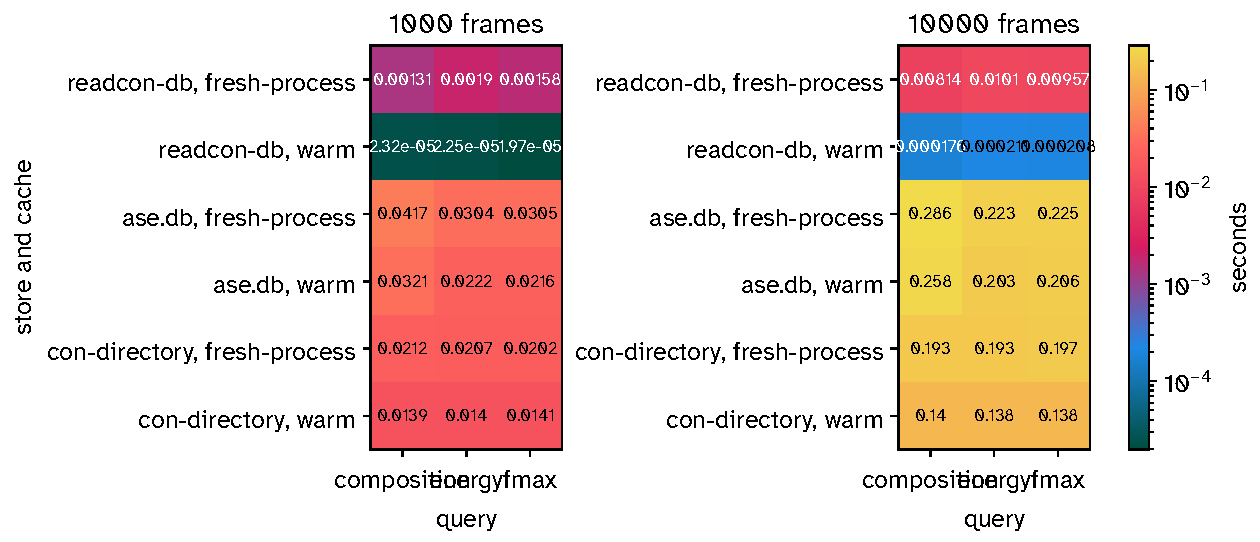
\includegraphics[width=\textwidth]{figures/generated/db_query_latency.pdf}
\caption{Median query time for composition, energy and maximum force, from the stored measurements.
Each panel is one corpus size.
Rows pair the store with a fresh process, cache left in place, or with the next query in that process.
The page cache was not dropped.}
\label{fig:db-query}
\end{figure}

readcon-db occupies 2.50 times the raw CON text, at both 1,000 and 10,000 frames.
The ASE database is smaller than the raw text.
Figure \ref{fig:db-disk} also shows gzip and zstd of the same text.

\begin{figure}[ht]
\centering
\includegraphics[width=\textwidth]{figures/generated/db_disk_footprint.pdf}
\caption{Allocated bytes for the raw text, two compressed copies, readcon-db, both ASE database files and a directory of 64-frame chunks.
The readcon-db cell is the memory-mapped file, text plus indexes.}
\label{fig:db-disk}
\end{figure}

One adaptive kinetic Monte Carlo trace of 24,000 frames stores 27.9 MB of blobs, \(27{,}864{,}917\) bytes, equal to the raw file, because the stored texts are kept separately.
The hash index of that stored trace records 7 unique structures, and their text is 8319 bytes.
Those seven texts are the unhopped hydrogen cyanide state and its saddle, the unhopped copper state and its saddle, and both platinum-hydrogen states together with that saddle.
Figure \ref{fig:db-dedup} compares the full trace with that unique set.
That collapse is a property of the repeated states in the trace.
It is separate from the campaign-band query in Section \ref{sec:supp-dedup}, which found no shared hash.

\begin{figure}[ht]
\centering
\includegraphics[width=0.85\textwidth]{figures/generated/db_dedup.pdf}
\caption{The stored 24{,}000-frame trace against its 7 unique structures.
The left panel counts frames.
The right panel is allocated bytes for the full corpus and for a corpus of the unique texts.}
\label{fig:db-dedup}
\end{figure}

Nine correctness checks pass on that store.
They cover a round trip, identical bytes sharing one hash entry, a one-digit coordinate change, a missing force or velocity section, periodicity taken only from the declared mask, a rebuild of the indexes from the stored text, a second rebuild, an ignored numeric cache, and a hash entry that remains after a duplicate is rewritten.
In readcon-db 0.1.8 the map starts at 2 GiB.
The caller can raise that limit, and a full map grows and retries.
These tables were collected with that 2 GiB ceiling, so one million frames exceed it.
A \(100{,}000\)-frame ingest was left out of the timed table, because the ASE database at 207 frames/s exceeds two minutes.
gzip and zstd in Figure \ref{fig:db-disk} are wrappers of the CON text.
The store keeps each text, so the stored blob bytes of the \(24{,}000\)-frame trace equal the raw file, and the indexes sit beside that text.
\section{Language pairs}
\label{sec:supp-pairs}
Table \ref{tab:restart-pairs} is the climbing-image band through each writer and reader among Python, C, C++, Fortran and Julia. Each pair reads the restart file written by the other.
% Written by paper/cpc/scripts/gen_cloud_tables.py.
\begin{table}[ht]
\centering
\scriptsize
\caption{Harness result for the same climbing-image band through each writer and reader among Python, C, C++, Fortran and Julia. The columns are the columns of Table~\ref{tab:restartfmt}.}
\label{tab:restart-pairs}
\setlength{\tabcolsep}{3pt}
\resizebox{\textwidth}{!}{%
\begin{tabular}{@{}lccccc@{}}
\toprule
Route & File (\AA) & Modes & Steps & $\Delta E^\ddagger$ (eV) & Max displacement (\AA) \\
\midrule
CON 3.1 Python to Python & 0 & 56 & 60 & $-2.31\times10^{-14}$ & $3.55\times10^{-15}$ \\
CON 3.1 Python to C & 0 & 56 & 60 & $-2.31\times10^{-14}$ & $3.55\times10^{-15}$ \\
CON 3.1 Python to C++ & 0 & 56 & 60 & $-2.31\times10^{-14}$ & $3.55\times10^{-15}$ \\
CON 3.1 Python to Fortran & 0 & 56 & 60 & $-2.31\times10^{-14}$ & $3.55\times10^{-15}$ \\
CON 3.1 Python to Julia & 0 & 56 & 60 & $-2.31\times10^{-14}$ & $3.55\times10^{-15}$ \\
CON 3.1 C to Python & 0 & 56 & 60 & $-2.31\times10^{-14}$ & $3.55\times10^{-15}$ \\
CON 3.1 C to C & 0 & 56 & 60 & $-2.31\times10^{-14}$ & $3.55\times10^{-15}$ \\
CON 3.1 C to C++ & 0 & 56 & 60 & $-2.31\times10^{-14}$ & $3.55\times10^{-15}$ \\
CON 3.1 C to Fortran & 0 & 56 & 60 & $-2.31\times10^{-14}$ & $3.55\times10^{-15}$ \\
CON 3.1 C to Julia & 0 & 56 & 60 & $-2.31\times10^{-14}$ & $3.55\times10^{-15}$ \\
CON 3.1 C++ to Python & 0 & 56 & 60 & $-2.31\times10^{-14}$ & $3.55\times10^{-15}$ \\
CON 3.1 C++ to C & 0 & 56 & 60 & $-2.31\times10^{-14}$ & $3.55\times10^{-15}$ \\
CON 3.1 C++ to C++ & 0 & 56 & 60 & $-2.31\times10^{-14}$ & $3.55\times10^{-15}$ \\
CON 3.1 C++ to Fortran & 0 & 56 & 60 & $-2.31\times10^{-14}$ & $3.55\times10^{-15}$ \\
CON 3.1 C++ to Julia & 0 & 56 & 60 & $-2.31\times10^{-14}$ & $3.55\times10^{-15}$ \\
CON 3.1 Fortran to Python & 0 & 56 & 60 & $-2.31\times10^{-14}$ & $3.55\times10^{-15}$ \\
CON 3.1 Fortran to C & 0 & 56 & 60 & $-2.31\times10^{-14}$ & $3.55\times10^{-15}$ \\
CON 3.1 Fortran to C++ & 0 & 56 & 60 & $-2.31\times10^{-14}$ & $3.55\times10^{-15}$ \\
CON 3.1 Fortran to Fortran & 0 & 56 & 60 & $-2.31\times10^{-14}$ & $3.55\times10^{-15}$ \\
CON 3.1 Fortran to Julia & 0 & 56 & 60 & $-2.31\times10^{-14}$ & $3.55\times10^{-15}$ \\
CON 3.1 Julia to Python & 0 & 56 & 60 & $-2.31\times10^{-14}$ & $3.55\times10^{-15}$ \\
CON 3.1 Julia to C & 0 & 56 & 60 & $-2.31\times10^{-14}$ & $3.55\times10^{-15}$ \\
CON 3.1 Julia to C++ & 0 & 56 & 60 & $-2.31\times10^{-14}$ & $3.55\times10^{-15}$ \\
CON 3.1 Julia to Fortran & 0 & 56 & 60 & $-2.31\times10^{-14}$ & $3.55\times10^{-15}$ \\
CON 3.1 Julia to Julia & 0 & 56 & 60 & $-2.31\times10^{-14}$ & $3.55\times10^{-15}$ \\
\bottomrule
\end{tabular}}
\end{table}

\section{MPI ranks}
\label{sec:supp-mpi}
Tables \ref{tab:mpi-strong} and \ref{tab:mpi-weak} in the main text are the warm medians.
The tables here list every rank that was run, cold and warm.
Ranks 16 and 32 were not run.
Every repeat matched the serial bytes.
\input{figures/generated/mpi_strong_cold}
\input{figures/generated/mpi_strong_warm_full}
\input{figures/generated/mpi_weak_cold}
\input{figures/generated/mpi_weak_warm_full}
\section{Records beside the checkpoint}
\label{sec:supp-neighbours}
Table \ref{tab:compare} answers four questions for the checkpoint and for the records that sit beside a saddle search.
Restart-exact means binary64 coordinates, the per-axis mask, the persistent identifier and the periodic flags all come back.
Velocities means a velocity block whose time unit is written in the file.
Metadata means a version or a schema a second reader can apply.
Indexed means frame \(k\) can be opened without a scan whose length is the number of earlier frames.
The first six rows are the round trips in Table \ref{tab:survey}.
Rows below the second rule are what the cited specification stores.

\begin{table}[ht]
\centering
\scriptsize
\caption{Restart record against neighbouring records.
The first six rows are measured in Table \ref{tab:survey}.
Later rows follow the cited specification.
``Scan'' means the reader walks the file to find a frame.
``Offsets'' means the reader records a byte offset after that scan, which stays serial because each start depends on the counts before it.}
\label{tab:compare}
\setlength{\tabcolsep}{4pt}
\begin{tabular}{@{}p{0.34\linewidth}llll@{}}
\toprule
Record & Restart-exact & Velocities & Metadata & Indexed \\
\midrule
CON 3.1 & yes & declared & versioned & offsets \\
extended XYZ & no & omitted & comment & scan \\
ASE trajectory & coordinates & unnamed & code & yes \\
POSCAR & mask changed & omitted & selective & no \\
H5MD & single precision & declared & versioned & HDF5 \\
ASE eon on CON & collapsed & rejected & none & no \\
\midrule
TNG, GROMACS, CHARMM, AMBER/NetCDF \cite{spangbergTrajectoryNgPortable2011,lundborgEfficientExtensibleFormat2014,abrahamGromacsHighPerformance2015,brooksCharmmBiomolecularSimulation2009,caseAmberBiomolecularSimulation2005,rewNetcdfInterfaceScientific1990} & trajectory & MD fields & container & frames \\
PDB, wwPDB, mmCIF \cite{bermanProteinDataBank2000,bermanAnnouncingWorldwideProtein2003,westbrookStarmmcifOntologyMacromolecular2000} & archive & omitted & ontology & archive id \\
LAMMPS, Atomsk, Open Babel \cite{thompsonLammpsFlexibleSimulation2022,hirelAtomskToolManipulating2015,oboyleOpenBabelOpen2011} & columns & deck units & converter & no \\
cclib, IOData, TREXIO, QCArchive \cite{oboyleCclibLibraryPackageindependent2008,verstraelenIodataPythonLibrary2021,posenitskiyTrexioFileFormat2023,smithMolssiQcaRchive2021} & QC object & omitted & schema & result index \\
OPTIMADE, NOMAD, Catalysis-Hub, Transition1x, OC20 \cite{andersenOptimadeApiExchanging2021,draxlNomadLaboratoryData2019,wintherCatalysishuborgOpenElectronic2019,schreinerTransition1xDatasetBuilding2022,chanussotOpenCatalyst20202021} & published geometry & omitted & schema & yes \\
MDTraj, VMD, OVITO, d-SEAMS, essential dynamics, MPI H5MD \cite{mcgibbonMdtrajModernOpen2015,humphreyVmdVisualMolecular1996,stukowskiVisualizationAnalysisAtomistic2010,goswamiDseamsDeferredStructural2020,meyerEssentialDynamicsTool2006,jakupovicMpiparallelMolecularDynamics2021} & analysis & from the file & the tool & opened file \\
Zarr, ADIOS2, portable scientific data \cite{opengeospatialconsortiumZarrStorageSpecification2022,godoyAdios2Adaptable2020,brownSoftwarePortableScientific1993} & arrays & omitted & container & chunks \\
PACKMOL \cite{martinezPackmolPackageBuilding2009} & initial box & omitted & none & no \\
PLUMED, ESPResSo \cite{tribelloPlumed2New2014,weikEspresso40Extensible2019} & program state & program & checkpoint & no \\
i-PI, MDI \cite{ceriottiIpiPythonInterface2014,kapilIpi20Universal2019,litmanIpi30Flexible2024,barnesMolssiDriverInterface2021} & live step & in the step & interface & no \\
\bottomrule
\end{tabular}
\end{table}

\section{Second Python thread sweep}
\label{sec:supp-threads}
The five-repeat pool sweep in Section \ref{sec:perf-read} and the thirty-pair sweep here are different campaigns on the same \(10{,}000\)-frame file.
The thirty-pair one-thread median is \(1.35258\,\mathrm{s}\).
Two threads give speedup \(1.148\) with interval \([1.126, 1.157]\), four give \(1.209\) with \([1.194, 1.223]\), and eight give \(1.284\) with \([1.263, 1.313]\).
The five-repeat Python speedup at eight threads is \(1.15\).
Both numbers stand.
The file read itself, measured by sending the bytes to the null device, has median \(0.018511\,\mathrm{s}\), \(9059.8\,\mathrm{MB/s}\).
Reading the bytes in the process takes \(0.094481528\,\mathrm{s}\), and scanning frame boundaries takes \(0.034419954\,\mathrm{s}\).
Their sum is \(0.128901482\,\mathrm{s}\), which is \(0.266523\) of the 15-repeat one-thread median \(0.483640922\,\mathrm{s}\).
That quotient is not the serial fraction of Figure \ref{fig:roofline}.
The figure has no Amdahl curve.

\section{ABNF of one frame}
\label{sec:appendix-abnf}
The non-normative ABNF of one frame follows.
An empty first header line is the user line, an empty second header line is implicit version 1, and a blank line after a frame is the next frame unless it begins a velocity block.
The listing has 50 rules.
The specification wins where the two disagree.
\input{figures/generated/con_abnf}

\section{Reproduction}
\label{sec:supp-repro}
The commands below rewrite every table and figure in the manuscript from the committed measurements.
They do not repeat the wall-clock campaigns.
Thread, peer and MPI timings were taken with \texttt{OMP\_NUM\_THREADS=1}, \texttt{OPENBLAS\_NUM\_THREADS=1} and \texttt{MKL\_NUM\_THREADS=1}.
The thread and peer-A binaries were built with rustc 1.88.0 and g++ 13.3.0.
Peer campaign B and the MPI binaries were built with rustc 1.99.0.
The store evaluation used rustc 1.88.0.
Run the commands from the repository root.

\begin{lstlisting}[caption={Rebuild of the manuscript tables and figures.},label={lst:repro}]
python3 paper/cpc/scripts/gen_tables.py
python3 paper/cpc/scripts/gen_cloud_tables.py
python3 paper/cpc/scripts/gen_failure_tables.py
python3 paper/cpc/scripts/file_sizes.py
python3 paper/cpc/scripts/trace_claimed.py
python3 paper/cpc/scripts/gen_figures.py
python3 paper/cpc/scripts/plot_figures.py
python3 paper/cpc/scripts/plot_supp.py
python3 paper/cpc/scripts/plot_restart_formats.py
python3 paper/cpc/scripts/plot_mpi_cloud.py
\end{lstlisting}

\texttt{gen\_tables.py} writes the peer table, the ratio table, the HCN table and the macro file.
\texttt{gen\_cloud\_tables.py} writes the restart tables and the MPI rank tables.
\texttt{gen\_failure\_tables.py} writes the survey, the extended-XYZ drift table and the version-safety table.
\texttt{file\_sizes.py} writes the byte-cost table.
\texttt{trace\_claimed.py} writes the weak-scaling rate table.
\texttt{gen\_figures.py} writes the architecture figure and the ABNF listing.
\texttt{plot\_figures.py} writes the Morse restart, the layer rates, the scaling rates, the mask bands and the store figures.
\texttt{plot\_supp.py} writes the restart-difference heatmap, the fidelity matrix, the frame anatomy, the velocity step, the illegal-file classes, the hash graph and the five-band maps.
\texttt{plot\_restart\_formats.py} writes the three resumed-band panels.
\texttt{plot\_mpi\_cloud.py} writes the strong-scaling and weak-scaling figures.

\bibliographystyle{elsarticle-num}
\bibliography{rg_main}
\end{document}
